\documentclass[10pt,a4paper]{article}
\PassOptionsToPackage{hyphens}{url}\usepackage{hyperref} 
\usepackage{draftcopy,epsfig,epsf,
,times,mathptm,graphicx,color,fancyhdr,
layout,amssymb,xspace,setspace,amsmath,printlen}
\usepackage[compact]{titlesec}
\usepackage{rotating}
\usepackage[a4paper, right=2cm,left=2cm]{geometry}
%\providecommand{\href}[2]{#2}   
%
\onehalfspacing
%\singlespacing

%%% setup format 
\renewcommand{\topfraction}{0.9}	% max fraction of floats at top
\renewcommand{\bottomfraction}{0.8}	% max fraction of floats at bottom
\renewcommand{\floatpagefraction}{0.7}	% require fuller float pages
\renewcommand{\dblfloatpagefraction}{0.7}	% require fuller float pages

%\setlength{\topmargin}{-2.3cm}
%\setlength{\oddsidemargin}{0cm}
%\setlength{\marginparsep}{0pt}
%\setlength{\marginparwidth}{62pt}

%\textwidth=17.0cm
%\textheight=24.7cm
%%%%%
%\uselengthunit{mm}
 \message{The text height is \the\textheight} 
 \message{The text width  is \the\textwidth}

 \message{The paper  height is \the\paperheight} 
 \message{The paper  width  is \the\paperwidth} 

\newlength{\foo}
\setlength{\foo}{12pt}
\uselengthunit{mm}
\typeout  {\printlength{\foo}}

%\typeout{The paper  width  is \printlength{\paperwidth}}

\pdfpagewidth=\paperwidth
\pdfpageheight=\paperheight

\newcommand{\fix}[1]{\    {(\bf{FIX} }{\it #1})}

\newcommand{\fb}{{\xspace fb$^{-1}$}\xspace}

\newcommand{\srootb}{$S\sqrt{B}$\ }
\newcommand\met{\not\!\! E_{T}}
\newcommand{\et}{$E_T$\xspace}
\newcommand{\ETHZ}{ETH Z\"urich\xspace}
\newcommand{\unit}[1]{\ensuremath{\mathrm{\:#1}}}
\newcommand{\hilumi}{\ensuremath{\mathcal{L}=\text{10}^\text{34}\,\text{cm}^\text{$-$2}\,\text{s}^\text{$-$1}}\xspace}

\newcommand{\TeV}{\ensuremath{\mathrm{TeV}}\xspace}
\newcommand{\GeV}{\ensuremath{\mathrm{GeV}}\xspace}

%%%%%%%%%%%%%%%%%%%%
%  CMS-abbreviations:

\newcommand{\MUHAT}{{$0.87 \pm 0.23$}} %%% 5HPA Jul21
%\newcommand{\PH}{\ensuremath{H}\xspace} 
%\newcommand{\mH}{\ensuremath{m_{\PH}}}
\newcommand{\mH}{\ensuremath{m_{\mathrm{H}}}}
\newcommand{\CLs}{\ensuremath{\mathrm{CL_s}\xspace}}
\newcommand\Wbb   {\ensuremath{\PW\bbbar}}
\newcommand\Zbb   {\ensuremath{\cPZ\bbbar}}
\newcommand\Mbb   {\ensuremath{m(\mathrm{jj})}}
\newcommand{\zjets}{\ensuremath{Z+\text{jets}}\xspace}

%%%% add private newcommands here below

%%%% newcommands Boris
\newcommand{\ttv}{$t\bar{t}V$\xspace}
\newcommand{\ttw}{$t\bar{t}W$\xspace}
\newcommand{\ttz}{$t\bar{t}Z$\xspace}
\newcommand{\ttbar}{$t\bar{t}$\xspace}
\newcommand{\ttH}{$t\bar{t}H$\xspace}
\newcommand{\ttHbb}{$t\bar{t}H(\rightarrow b\bar{b})$\xspace}
\newcommand{\VH}{$VH$\xspace}
\newcommand{\VHbb}{$VH(\rightarrow b\bar{b})$\xspace}
\newcommand{\ttHWWZZ}{$t\bar{t}H(\rightarrow WW/ZZ)$\xspace}

\newcommand{\cmsSymbolFace}{\relax}
\newcommand{\PWm}{\ensuremath{{W^-}}}
\newcommand{\sTop}{\ensuremath{\widetilde{\cmsSymbolFace{t}}}\xspace}
\newcommand{\sBot}{\ensuremath{\widetilde{\cmsSymbolFace{b}}}\xspace}
\newcommand{\cPqt}{\ensuremath{\cmsSymbolFace{t}}} % t for t quark
\newcommand{\chim}{\ensuremath{\widetilde{\chi}^{-}}\xspace}
\newcommand{\chip}{\ensuremath{\widetilde{\chi}^{+}}\xspace}
\newcommand{\chiz}{\ensuremath{\widetilde{\chi}^{0}}\xspace}
\newcommand{\sGlu}{\ensuremath{\widetilde{\cmsSymbolFace{g}}}\xspace}
\newcommand {\vs}{\mbox{\sl vs.}\xspace}      %vs.

%%%% newcommands Grab, Luca
\newcommand{\gev}{\mathrm{GeV}} 
\newcommand{\mev}{\mathrm{MeV}} 
%\newcommand{\TeV}{\ensuremath{\mathrm{TeV}\xspace}}
%\newcommand{\GeV}{\ensuremath{\mathrm{GeV}\xspace}}
%\newcommand $13\,\textrm{TeV}$
\newcommand{\hgg}{\ensuremath{H{\rightarrow\,}\gamma\gamma}}
\newcommand{\hZZllllnostar}{\ensuremath{H{\rightarrow\,}ZZ{\rightarrow\,}4\ell}}
\newcommand{\Hlvlv}{H\to WW^*\to \ell\nu\ell\nu}
\newcommand{\Hllll}{H\to ZZ^*\to 4\ell}
\newcommand{\Htt}{H\to\tau\tau}
\newcommand{\Hbb}{H\to b\bar{b}}
\newcommand{\Hmm}{H\to \mu\mu}



\newcommand{\pbinv}{\rm\,pb^{-1}}
\newcommand{\xizero}{$\Xi(1530)^{0}\,$}
\newcommand{\bce}{\begin{center}}
\newcommand{\ece}{\end{center}}
\newcommand{\beqn}{\begin{eqnarray*}}
\newcommand{\eeqn}{\end{eqnarray*}}
\newcommand{\be}{\begin{equation}}
\newcommand{\ee}{\end{equation}}
\newcommand{\ed}{\end{displaymath}}
\newcommand{\bit}{\begin{itemize}}
\newcommand{\eit}{\end{itemize}}
\newcommand{\ben}{\begin{enumerate}}
\newcommand{\een}{\end{enumerate}}
\newcommand{\domm}{$D^0 \rightarrow \mu^+ \mu^- $}
\newcommand{\as}{\alpha_s}
\newcommand{\an}{\overline{\alpha}_0}
\newcommand{\mean}[1]{\left< #1 \right>}
\newcommand{\fmean}{\mean{F}}
\newcommand{\fpert}{\fmean^{\rm pert}}
\newcommand{\fpow}{\fmean^{\rm pow}}
\newcommand{\mr}{\mu_{\scriptscriptstyle R}}
\newcommand{\jrnl}[4]{{#1} {\bf #2} (#3) #4.}
\newcommand{\PLB}{{\em Phys.~Lett.\ }{\bf B}}
\newcommand{\dxphi}{$\Delta \Phi_{\rm{l-X}}$\,}
\newcommand{\anotop}{Anomalous Top Production\,}
\newcommand{\ptmiss}{$P_{T}^{\rm{miss}}$\,}
\newcommand{\pb}{$\rm{pb}^{-1}$}
\newcommand{\lumi}{\mathcal{L}}
\newcommand{\rphi}{$r\!-\!\phi$\,}
\newcommand{\rz}{$r\!-\!z$\,}
\newcommand{\um}{\,\mu\textrm{m}\,}
\newcommand{\pt}{$p_{\textrm{T}}$\,}
\newcommand{\cm}{\,\textrm{cm}\,}
\newcommand{\FL}{$ F_{L}(x,Q^2)\,$}
\newcommand{\Fc}{$ F_{2}\,$}
\newcommand{\FLc}{$ F_{L}\,$}
\newcommand{\F}{$ F_{2}(x,Q^2)\,$}
%\newcommand{\TeV}{\ensuremath{\mathrm{TeV}}\xspace}
%\newcommand{\GeV}{\ensuremath{\mathrm{GeV}}\xspace}
\newcommand{\MeV}{\ensuremath{\mathrm{MeV}}}
\newcommand{\keV}{\ensuremath{\mathrm{keV}}}
\newcommand{\pom}{\ensuremath{\Bbb{P}}}
\newcommand{\sub}[1]{\ensuremath{_{\mathrm{#1}}}}
\newcommand{\super}[1]{\ensuremath{^{\mathrm{#1}}}}
\newcommand{\der}{\ensuremath{\mathrm{d}}}
\newcommand{\mpipi}{\ensuremath{m_{\mathrm{\pi\pi}}}}
\newcommand{\mrho}{\ensuremath{m_{\mathrm{\rho}}}}
\newcommand{\Grho}{\ensuremath{\Gamma_{\mathrm{\rho}}}}
\newcommand{\Grhon}{\ensuremath{\Gamma_{\mathrm{\rho,0}}}}
%
\newcommand{\xgobs}{$x_{\gamma}^{\textrm{obs}}$}
\newcommand{\xgobsm}{x_{\gamma}^{\textrm{obs}}}
\newcommand{\ptjet}{$p_{\textrm{t}}^{\textrm{\,jet}_{1}}$}
%
\newcommand{\gevsq}{\,\mathrm{GeV}^2}
\newcommand{\gv}{~GeV$^2$}
\newcommand{\llam}{$\lambda(x,Q^2)\:$}
\newcommand{\lam}{$\lambda(Q^2)\:$}
\newcommand{\dst}{$D^{*+}$}
\newcommand{\dc}{$D^+$}
\newcommand{\dn}{$D^0$}
\newcommand{\ds}{$D^+_s$}
\newcommand{\mhpp}{\mbox{$M_H$}}
\newcommand{\hpp}{\mbox{$H^{\pm\pm}$}}
%\newcommand{\unit}[1]{\ {\rm#1}}
% high q2
\newcommand{\bs}{\bar{s}}
\newcommand{\bc}{\bar{c}}
\newcommand{\bu}{\bar{u}}
\newcommand{\bb}{\bar{b}}
\newcommand{\bU}{\bar{U}}
\newcommand{\bD}{\bar{D}}
\newcommand{\bd}{\bar{d}}
\newcommand{\bq}{\bar{q}}    
\newcommand{\wtwogen} {W_2}
\newcommand{\wlgen} {W_L}
\newcommand{\xwthreegen} {xW_3}
\newcommand{\Wtwo}   {\mbox{$W_2$}}
\newcommand{\Wz}   {\mbox{$W_3$}}
\newcommand{\WL}   {\mbox{$W_{_{L}}$}}
\newcommand{\QQ}  {\mbox{${Q^2}$}}

\newcommand{\alpset}{\alpha_s(E_T)}
\newcommand{\pqqc}{$\Xi^{--}_{5q}\,$}
\newcommand{\pqqn}{$\Xi^{0}_{5q}\,$}

\def\b     {\ensuremath{b\;}}
\def\bbar {\ensuremath{\overline b\;}}
\def\bbbar {\ensuremath{b\overline b\;}}
\def\B     {\ensuremath{B\;}}

%\newcommand{\bhadb}{\ensuremath{\mathrm{B}{\overline{\mathrm{B}}}}\xspace}
%\newcommand{\bbar}{\ensuremath{{\overline{\mathrm{b}}}}\xspace}
%\newcommand{\bbbar}{\ensuremath{\mathrm{b}{\overline{\mathrm{b}}}}\xspace}

\newcommand{\cbar}{\ensuremath{{\overline{\mathrm{c}}}}\xspace}
\newcommand{\CASCADE}{{\textsc{cascade}}\xspace}
\newcommand{\Pbquark}{\ensuremath{\mathrm{b}}\xspace}
\newcommand{\Pbbbar}{\ensuremath{\mathrm{b\overline{b}}}\xspace}



%\pagestyle{headings

%%%% 
%\includeonly{1Overview}
%\includeonly{2Higgs}
%\includeonly{3LHCsearches}
%\includeonly{4DiscussionSearches}
%\includeonly{5Flavour}
%\includeonly{6LowEnergy}
%\includeonly{7StandardModel}
%\includeonly{8Theory}
%\includeonly{9DiscussionConnections} 
%\includeonly{10Accelerators}
%\includeonly{11Detectors}
%\includeonly{12Summary} 
%\includeonly{13ConcludingRemarks}

\begin{document}
\addtocounter{page}{-1}
\pagestyle{plain}
%\layout                                                                            
%bla     
\begin{center}
{\large {\bf  SWHEPPS 2016:}\\
\ ~\\
Summary of the\\
 Strategic Workshop for High Energy Particle Physics \\
  in Switzerland }\\
\vspace{2cm}

 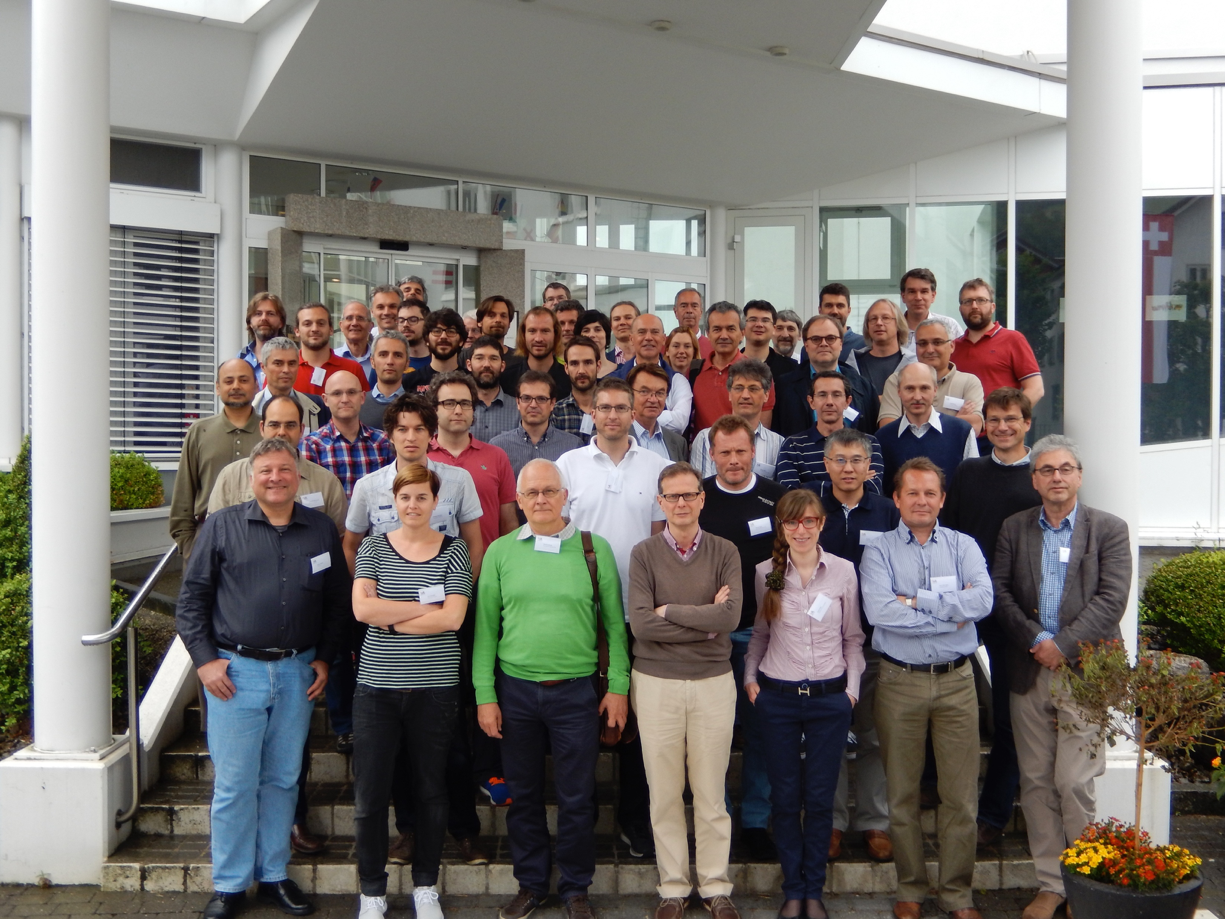
\includegraphics[width=0.5\textwidth]{figures/GroupPicture.png}
 
\vspace{6cm}

Seminarhotel Aegerisee, 7-9 June 2016 \\
\url{https://indico.cern.ch/event/504502/}  ~\\
\  ~\\


\vspace {-0.5cm}
 \begin{figure}[h]
   \centering
   
\includegraphics[width=0.1\textwidth]{figures/CHIPPlogo.png}
 \end{figure}

\vspace{-0.4cm}
\today \\
\end{center}
%\end{document}
\newpage 

%%%%%%%%%%%%%%%%%%%%%%%%%%%%%%
%  Workshop Overview
%
%  Editor: Rainer Wallny
%%%%%%%%%%%%%%%%%%%%%%%%%%%%%%
\section{Overview of the Workshop}\label{Overview}
\fix{editor: Rainer}



\noindent SWHEPPS~\cite{workshopindico},  the Strategic Workshop on High Energy Particle Physics in Switzerland, was a 2.5 day workshop that took place from 8-10 June 2016 at 
Seminarhotel Aegerisee.   It was  modeled as a plenary session-only retreat of primarily senior CH researchers and PIs engaged in CHIPP~\cite{chipp} pillar 1 activities, 
i.e. research at the high energy and low energy frontier (an introduction to the pillar structure of CHIPP can be found in the CHIPP roadmap~\cite{roadmap}). The aim  of the workshop
 was to take stock of the present state of the field in order to identify key elements influencing the strategy of Swiss researches active in pillar 1 research activities for the next 5-15 years or
 - failing that - define milestones when identifying those elements should become clearer. The workshop should furthermore serve as a kick-off meeting to start  process of editing a
 CHIPP whitepaper on future pillar 1 activities in order to  complement similar documents pertaining to the neutrino pillar~\cite{neutrinowhitepaper} and the astroparticle 
  pillar~\cite{astroparticlepillarwhitepaper} in time for the Update of the European Strategy for Particle Physics  of the  CERN council~\cite{europeanstrategy}. 



 


 

We would like the convenors to select and invite speakers for their session primarily from the CH community with the possibility to invite an external keynote speaker with paid expenses that could help to shape and sharpen the discussion.  Sessions are between 90min and 2 hours and presentations should be typically 25+5min. We leave it up to the convenors to arrange the details of their session but hope for a selection that takes regional balance into account. Attached you find a draft timetable that we have worked out. Convenors of experimental sessions can of course invite theoretical contributions if they deem fit, but should discuss those with the theory convenors and vice versa. This may be particularly relevant for your session to interact with
the "BSM physics I: SUSY and Exotics" session.

 

 At the end of each day, a 90min discussion session should allow for the exchange of ideas between all participants of the workshop, also  in view of the whitepaper.   We foresee a further role for the session convenors to act as potential editors of a section in the whitepaper and thus would hope that they also actively engage in the discussion session as well. 

 

Please let us know whether you would be willing to take over this important task, both for the workshop as well as the whitepaper editing. We would be delighted if we could hear from you ideally by early February.  Thank you very much for considering. Please do not hesitate to contact us with any questions. 


%%%%%%%%%%%%%%%%%%%%%%%%%%%%%%
%  Higgs Session
%
%  Editors: Florencia Canelli, Michele Weber
%%%%%%%%%%%%%%%%%%%%%%%%%%%%%%
\section{TemplateEntry}\label{Template}






%%%%%%%%%%%%%%%%%%%%%%%%%%%%%%
%  LHC Searches
%
%  Editors: Ben Kilminster, Tobias Golling
%%%%%%%%%%%%%%%%%%%%%%%%%%%%%%
\include{3LHCsearches}

%%%%%%%%%%%%%%%%%%%%%%%%%%%%%%
%  DiscussionSession Searches
%
%  Editors: Ben Kilminster, Tobias Golling
%%%%%%%%%%%%%%%%%%%%%%%%%%%%%%
\section{TemplateEntry}\label{Template}






%%%%%%%%%%%%%%%%%%%%%%%%%%%%%%
%  Flavour Physics
%
%  Editors: Olivier Schneider, Adrian Signer, Klaus Kirch
%%%%%%%%%%%%%%%%%%%%%%%%%%%%%%
\section{TemplateEntry}\label{Template}






%%%%%%%%%%%%%%%%%%%%%%%%%%%%%%
% Low Energy Physics 
%
%  Editors: Olivier Schneider, Adrian Signer, Klaus Kirch
%%%%%%%%%%%%%%%%%%%%%%%%%%%%%%
\section{TemplateEntry}\label{Template}






%%%%%%%%%%%%%%%%%%%%%%%%%%%%%%
% Standard Model Physics 
%
%  Editors: Florencia Canelli, Michele Weber 
%%%%%%%%%%%%%%%%%%%%%%%%%%%%%%
\section{TemplateEntry}\label{Template}







%%%%%%%%%%%%%%%%%%%%%%%%%%%%%%
% Theory including Connections 
%
%  Editors: Gino Isidori, Ricardo Rattazzi,  Thomas Gehrmann
%%%%%%%%%%%%%%%%%%%%%%%%%%%%%%
\section{TemplateEntry}\label{Template}






%%%%%%%%%%%%%%%%%%%%%%%%%%%%%%
% DiscussionSession: Connections 
%
%  Editors: Gino Isidori, Olivier Schneider 
%%%%%%%%%%%%%%%%%%%%%%%%%%%%%%
\section{TemplateEntry}\label{Template}




 

%%%%%%%%%%%%%%%%%%%%%%%%%%%%%%
% New Accelerators
%
%  Editors: Lenny Rivkin
%%%%%%%%%%%%%%%%%%%%%%%%%%%%%%
\section{TemplateEntry}\label{Template}






%%%%%%%%%%%%%%%%%%%%%%%%%%%%%%
% New Detectors
%
%  Editors: Roland Horisberger, Sergio Gonzales Sevilla
%%%%%%%%%%%%%%%%%%%%%%%%%%%%%%
\section{TemplateEntry}\label{Template}






%%%%%%%%%%%%%%%%%%%%%%%%%%%%%%
% DiscussionSession: New Accelerators and Facilties and Summary
%
%  Editors: Tatusya Nakada, Lenny Rivkin
%%%%%%%%%%%%%%%%%%%%%%%%%%%%%%
\section{TemplateEntry}\label{Template}




 

%%%%%%%%%%%%%%%%%%%%%%%%%%%%%%
%
%  ConcludingRemarks 
%   Editor: Rainer Wallny
%%%%%%%%%%%%%%%%%%%%%%%%%%%%%%
\include{13ConcludingRemarks}



%%%%%%%%%%%%%%%%%%%%%%%%%%%%%%
%
%Bibliography 									
%
%%%%%%%%%%%%%%%%%%%%%%%%%%%%%%
%\onehalfspacing
\singlespacing

\begin{thebibliography}{100}
\bibitem{workshopindico} The conference website can be found here: \url{https://indico.cern.ch/event/504502/}

\bibitem{chipp} The Swiss Institute of Particle Physics CHIPP is an institution under Swiss law, see \url{http://www.chipp.ch/}.

\bibitem{roadmap}  Roadmap of CHIPP \url{http://www.chipp.ch/chipp-meet-roadmap.html}


\bibitem{neutrinowhitepaper}  "Experimental neutrino physics: Switzerland in the global context, a white paper, 14. November 2015, 
\url{http://www.chipp.ch/documents/neutrino_whitepaper_14Nov2015_approved.pdf}

\bibitem{astroparticlepillarwhitepaper} "Strategy for Swiss contributions to large ground-based astro-particle physics research infrastructure", 17. March 2013, 
\url{http://www.chipp.ch/documents/astroparticle_whitepaper_17Mar2013_approved.pdf}

\bibitem{europeanstrategy} See \url{http://council.web.cern.ch/council/en/EuropeanStrategy/ESParticlePhysics.html}.

\bibitem{ATLASCMScouplings} 
The ATLAS and CMS Collaborations,
  ``Measurements of the Higgs boson production and decay rates and constraints on its couplings from a combined ATLAS and CMS analysis of the LHC pp collision data at $\sqrt{s} =$ 7 and 8 TeV,''
  \url{https://cds.cern.ch/record/2053103}
  %CMS-PAS-HIG-15-002.

\bibitem{lhc:rrb} ``Status and Plans for the LHC and the Experiments'' presented by Sergio Bertolucci, October 2014\\
\url{http://indico.cern.ch/event/334150/session/0/contribution/1/attachments/652322/896966/RRB_October14_SB.pdf}

\end{thebibliography}
%%%%% CLEAR DOUBLE PAGE!
\newpage{\pagestyle{empty}\cleardoublepage}






\end{document}
